\documentclass{bmcart}

%%%%%%%%%%%%%%%%%%%%%%%%%%%%%%%%%%%%%%%%%%%%%%
%%                                          %%
%% CARGA DE PAQUETES DE LATEX               %%
%%                                          %%
%%%%%%%%%%%%%%%%%%%%%%%%%%%%%%%%%%%%%%%%%%%%%%

%%% Load packages
\usepackage{amsthm,amsmath}
\usepackage{graphicx}
%\RequirePackage[numbers]{natbib}
%\RequirePackage{hyperref}
\usepackage[utf8]{inputenc} %unicode support
%\usepackage[applemac]{inputenc} %applemac support if unicode package fails
%\usepackage[latin1]{inputenc} %UNIX support if unicode package fails


%%%%%%%%%%%%%%%%%%%%%%%%%%%%%%%%%%%%%%%%%%%%%%
%%                                          %%
%% COMIENZO DEL DOCUMENTO                   %%
%%                                          %%
%%%%%%%%%%%%%%%%%%%%%%%%%%%%%%%%%%%%%%%%%%%%%%

\begin{document}

	\begin{frontmatter}
	
		\begin{fmbox}
			\dochead{Research}
			
			%%%%%%%%%%%%%%%%%%%%%%%%%%%%%%%%%%%%%%%%%%%%%%
			%% INTRODUCIR TITULO PROYECTO               %%
			%%%%%%%%%%%%%%%%%%%%%%%%%%%%%%%%%%%%%%%%%%%%%%
			
			\title{Interaccion a nivel molecular hospedador-virus del SARS-CoV2}
			
			%%%%%%%%%%%%%%%%%%%%%%%%%%%%%%%%%%%%%%%%%%%%%%
			%% AUTORES. METER UNA ENTRADA AUTHOR        %%
			%% POR PERSONA                              %%
			%%%%%%%%%%%%%%%%%%%%%%%%%%%%%%%%%%%%%%%%%%%%%%
			
			\author[
			  addressref={aff1},                   % ESTA LINEA SE COPIA IGUAL PARA CADA AUTOR
			  corref={aff1},                       % ESTA LINEA SOLO DEBE TENERLA EL COORDINADOR DEL GRUPO
			  email={emanuelamariastoia@gmail.com}   % VUESTRO CORREO ACTIVO
			]{\inits{E.M.S}\fnm{Emanuela Maria} \snm{Stoia}} % inits: INICIALES DE AUTOR, fnm: NOMBRE DE AUTOR, snm: APELLIDOS DE AUTOR
			\author[
			  addressref={aff1},
			  email={joseantoniomr99@gmail.com}
			]{\inits{J.A.M}\fnm{Jose Antonio} \snm{Muñoz}}
			\author[
			  addressref={aff1},
			  email={stephancharles1999@yahoo.es}
			]{\inits{S.C.N}\fnm{Stephan Charles} \snm{Nielson}}
			
			%%%%%%%%%%%%%%%%%%%%%%%%%%%%%%%%%%%%%%%%%%%%%%
			%% AFILIACION. NO TOCAR                     %%
			%%%%%%%%%%%%%%%%%%%%%%%%%%%%%%%%%%%%%%%%%%%%%%
			
			\address[id=aff1]{%                           % unique id
			  \orgdiv{ETSI Informática},             % department, if any
			  \orgname{Universidad de Málaga},          % university, etc
			  \city{Málaga},                              % city
			  \cny{España}                                    % country
			}
		
		\end{fmbox}% comment this for two column layout
		
		\begin{abstractbox}
		
			\begin{abstract} % abstract
			
			%%%%%%%%%%%%%%%%%%%%%%%%%%%%%%%%%%%%%%%%%%%%%%%
			%% RESUMEN BREVE DE NO MAS DE 100 PALABRAS   %%
			%%%%%%%%%%%%%%%%%%%%%%%%%%%%%%%%%%%%%%%%%%%%%%%	
			
			En este proyecto de investigacion se lleva a cabo una expansion en red, de una red de interaccion entre proteinas de Covid y proteinas 				humanas. 
			Esta expansion se llevara acabo buscando las rutas entre proteínas humanas usando el paquete de igraph. Esto es util para la 					biología se sistemas, donde vimos no era suficiente un analisis reduccionista sino una vision holistica.
			Esta vision nos permitira ver la influencia del covid en un organismo humano viendo todas las proteinas afectadas, y no solamente los 				primeros enlaces. Pudiendo hacer un analisis funcional para ver las funciones a las que afecta. 
			
			
			\end{abstract}
			
			%%%%%%%%%%%%%%%%%%%%%%%%%%%%%%%%%%%%%%%%%%%%%%
			%% PALABRAS CLAVE DEL PROYECTO              %%
			%%%%%%%%%%%%%%%%%%%%%%%%%%%%%%%%%%%%%%%%%%%%%%
			
			\begin{keyword}
			\kwd{rutas}
			\kwd{proteinas}
			\kwd{nodos}
			\kwd{red}
			\kwd{interaccino}
			\kwd{covid}
			\kwd{proteoma}
			\kwd{grafo}
			\kwd{enlaces}
			\end{keyword}
		
		
		\end{abstractbox}
	
	\end{frontmatter}	
	
	%%%%%%%%%%%%%%%%%%%%%%%%%%%%%%%%%
	%% COMIENZO DEL DOCUMENTO REAL %%
	%%%%%%%%%%%%%%%%%%%%%%%%%%%%%%%%%
	
	\section{Introducción}
\begin{document}
Tal y como nos muestra la biología de sístemas, sabemos que un organismo biológico es un sistema integrado e iterrelacionado de genes,
proteínas y reacciones bioqímicas, que da lugar a procesos biológicos. Nuestro estudio consiste en ver la relación de los genes viricos 
pertenecientes al SARS-CoV2 con los genes humanos. Partimos de alrededor de 30 grafos individuales, que muestra la proteina virica y los
patógenos unidos a las proteínas humanas. Estos datos al ser descargados nos ofrecen seis ficheros .xslx que muestra el nombre en uniprot, 
symbol de estas proteinas humanas, junto con algunas descripciones. Nuestros ficheros de interés son Network_table.xlsx y Prey_Lookup_Table.xlsx, 
analizaremos estos datos y veremos cuál nos será útil para el trabajo que queremos llevar a cabo. Nuestro objetivo es tomar cada uno de estos grafos
y unirlos entre sí mediante interacciones proteínahumana-proteinahumana, para conseguir un único grafo conexo completo.
Para esto usaremos la red del proteoma humano conseguida en string "9606.protein.links.v11.5.txt".
\end{document}

	\section{Materiales y métodos}


\subsection{Obtención de datos en formato String}
En este estudio debemos realizar una ampliacion de la red de proteinas humanas unidas a proteinas viricas.
Esta ampliacion debe hacerse usando una red de string, que emplea codigo ensamble para nombrar a las proteinas.
Nuestros datos están codificados con symbol o Uniprot. Por tanto, debemos hacer un cambio de esta codificacion a ensamble.
Para esto hemos empleado tres metodos, y nos quedaremos con aquel que nos permita trabajar con el mayor numero de genes humanos unidos a los genes del covid.
Los métodos empleados son: bitR, biomaRt, y utilizar una tabla obtenida de la base de datos de uniprot. 

\subsection{Obtención del grafo de relaciones proteinascovid-proteinasHumanas}
Antes de abordar un problema con la gran cantidad de datos que tiene (11 millones de datos el proteoma humano), hemos creado el codigo JugarRedes.R, donde hemos creado dos dataframe con pocos datos, y dos objetos igraph para poder ir probando las diferentes funciones y formas de obtener el grafo. Una vez familiarizados con las funciones y trabajar con listas hemos pasado a la implementacion del grafo de unica componente conexa.
Para la realizacion del grafo con una unica componente conexa, donde se forme la red minima del interactoma humano
que permita conectar todas las proteínas viricas del SARS-CoV2, hemos usado las funciones all\_simple\_paths y all\_shortest\_paths 
del paquete igraph de R. Debido al gran tamaño de la red y a las miles de combinaciones posibles, obteniamos caminos enormes que
se han abordado realizando pequeñas modificaciones que nos permita obtener la componente conexa con un tiempo de ejecucion y 
uso de memoria razonable. 

\subsection{Comparacion entre la red obtenida y la red humana}
Usando funciones del paquete igraph se han analizado ciertas propiedades de ambas redes para poder compararlas. 
Las propiedades analizadas son: densidad, reprocidad, diametro, grado, distribucion de grado, distancia media y asortatividad.

\subsection{Obtencion de la modularidad}
Para estudiar la modularidad del grafo obtenido hemos utilizado unicamente el paquete iGraph, ya que su combinacion de funciones nos permite obtener justo lo que necesitamos.
En este caso, las funciones principales son cluster\_walktrap y modularity. Cluster\_walktrap encontrara los subgrafos o comunidades en nuestro grafo a traves de recorridos aleatorios, y modulatiry calculara la modularidad a partir de ellos. 
A parte, la funcion communities me ha permitido ver claramente los grupos, y posteriormente representarlos con plot.igraph.

\subsection{Obtencion de la centralidad}
La centralidad determina la importancia que puede obtener un nodo dentro de una red, sin embargo, esta importancia puede medirse de numerosas formas, siendo algunas de ellas m\'as correctas en ocasiones que otras.
Con el objetivo de estudiar la centralidad de nuestra red, se ha decidido emplear los paquetes \textbf{igraph} y \textbf{CINNA} principalmente. Adem\'as, se ha utilizado un sistema m\'as simple pero que forma una sola componente conexa, debido al alto costo de computaci\'on que tiene el formar una sola componente conexa con todos los nodos que tenemos.
Mediante el paquete CINNA hemos decidido comprobar la centralidad que se obtiene mediante algunos de los metodos mas comunes como pueden ser el algoritmo \textbf{page-rank}, centralidad mediante el grado de cada \textbf{nodo}, la centralidad basada en la \textbf{cercania} y la centralidad a traves del \textbf{betweeness}(capacidad para estar en medio de los paths biologicos importantes).
Para obtener el m\'etodo de centralidad que sea considerado m\'as adecuado en nuestro caso, realizaremos una \textbf{pca}(an\'alisis de componentes) en la que se ver\'a reflejada la participaci\'on de cada medida de modularidad en nuestros datos. De esta manera podremos coger el método más adecuado para estos datos.

\subsection{Obtencion de la robustez}
Para obtener una medida de la robustez de nuetro grafo hemos realizado dos ataques dirigido. Para ambos hemos usado la funcion robustness del paquete brainGraph, la unica variacion es el parametro que determina el tipo de ataque, dado que realizamos un ataque basado en degree y otro en betweenness. Luego las hemos representado con un plot para una mejor visualizacion.

\subsection{Enriquecimiento funcional}
Nos ha parecido importante realizar un enriquecimiento funcional de los genes para ver en que funciones participan los genes del subgrafo utilizado en anteriores apartados.\newline
Para ello, contaremos con dos paquetes que ser\'an \textbf{clusterProfiler} y \textbf{biomaRt}. Pensamos usar \textbf{GO}(Gene Ontology) para poder obtener las funciones de los genes, sin embargo, en \textit{GO} hay tres tipos de t\'erminos que podemos obtener de los genes. Estos tres tipos son los procesos biol\'ogicos en los que est\'an implicados los genes, las funciones moleculares que realizan y los componentes celulares con los que tienen relaci\'on.\newline
Gracias a la funci\'on \textbf{enrichGO} de \textit{clusterProfiler}, podremos obtener esas tres informaciones de una manera sencilla. Sin embargo, los genes con los que trabaja dicha funci\'on tienen que estar en formato \textbf{ENTREZID}.\newline
Como nuestros datos est\'an en formato \textbf{ENSEMBLPROT}, tendremos que cambiarles la notaci\'on. Es por ello que tambi\'en se utilizar\'a biomaRt, de forma que buscaremos en la base de datos \textbf{genes} que contiene un dataset de genes humanos en formato \textit{ENSEMBLPROT}. En dicho dataset tambi\'en se encuentran todos los genes en formato \textit{ENTREZID}. Una vez teniendo la conexi\'on a dicha base de datos mediante \textit{biomaRt}, ser\'a sencillo pasarlos al formato requerido.\newline
Cabe decir que, en un principio se pensaba utilizar la funci\'on \textbf{bitr} perteneciente tambi\'en a \textit{clusterProfiler} pero debido a que el m\'etodo estaba desfasado y que no consegu\'ia emparejar el 84\% de los genes, se acab\'o por descartar y usar \textit{biomaRt}.

	
\section{Resultados}

\subsection{Obtencion de datos en formato String}
Se utilizan los tres metodos mencionados en la seccion de Materiales y Metodos.

\subsubsection{bitR}
Para este analisis hemos usado el paquete bitR de Rstudio. Hemos realizado un bitR del proteoma humano para un score maayor de 650. Posteriormente hemos comprobado cuantas de las proteinas humanas de nuestra tabla de union con covid se encuentra en nuestro proteoma obtenido. Posteriormente, hemos comprobado cuantas de ellas estan unidas a genes covid, y cuantos genes covid son.

\subsubsection{biomaRt}
Para este analisis hemos utilizado un paquete de Rstudio llamado biomaRt. Este paquete nos permite cambiar la codificacion de uniprot a ensamble.
El codigo perteneciente a este analisis se encuentra en la carpeta code y se denomina biomart.R. En este codigo viene detallado con comentarios el
proceso que se ha llevado a cabo. Basicamente los pasos seguidos son: 
- pasar de codigo uniprot a ensamble
- comprobar cuantos de estos codigos ensamble se encuentran en el proteoma completo, guardamos en un dataframe los valores ensamble y uniprot.  Comprobamos que solo nos quedamos de 332 proteinas humanas unidas a viricas con 107.
- Hacemos un bucle y guardamos en un dataframe los valores de uniprot y ensamble aquellos que coinciden con nuestra tabla de entrada.
- Hacemos un merge que nos une los dos dataframe, el de entrada con genes covid y humanos, y el obtenido con el cambio de uniprot a ensamble. 


\subsubsection{Tabla UniProt}
Para este analisis hemos utilizado una tabla obtenida de la base de datos de UniProt, que contiene tres columnas. Un valor de uniprot, uno de ensamble y otro tipo de codigo uniprot para el mismo gen. 
El codigo perteneciente a este analisis se encuentra en la carpeta code y se denomina tablaObtenidaUniprot.R. Nuevamente en el codigo vienen detallados los pasos seguidos. 
El proceso llevado a cabo es el siguiente:
- Leemos los ficheros: la tabla de uniprot, la tabla de relaciones entre genes viricos y humanos, y el proteoma de interaccion completo. El fichero con la tabla de uniprot tiene filas que no contienen codigo ensamble para algunos de los genes. Asi que realizaremos un filtrado que elimine estas filas.
- Una vez realizado esto, buscaremos cuantos de estos codigos ensamble se encuentran en el proteoma completo. Vemos que solo perdemos cuatro de estos codigos.
- Posteriormente, buscaremos cuantos de los codigos uniprot de mi tabla de entrada podemos convertir a ensamble. 


\subsection{Obtencion del grafo de relaciones proteinascovid-proteinasHumanas}

Para abordar el problema de la creacion de un grafo conexo, nos hemos enfrentado a tiempos de ejecucion elevados y un gasto de memoria elevada. 
El codigo denominado AlgoritmoRedCompleta.R muestra como se ha llevado a cabo el proceso de obtencion de red. 
Una vez obtenido en el apartado anterior la tabla con nuestros genes uniprot en formato string, ya podriamos usar funciones pertenecientes a igraph que buscaran rutas entre una y otra proteina humana dentro del proteoma. 
Como primer paso se intento obtener todas las rutas posibles entre todas las proteinas humanas unidas al covid, usando la función all simple paths. 
Nos enfrentamos a una compilacion donde tras 15 horas de ejecucion continua nuestro código no había terminado de definir las rutas entre las proteinas,además de haber generado un archivo de casi 15 gigas que por poco ocupaba toda la memoria de R. 
Decidimos hacer una pequeña modificaciones y calcular todas las rutas posibles con la misma funcion pero simplemente haciendo las combinaciones de un gen con su siguiente. Nuevamente el tiempo de ejecucion y la memoria ocupada eran inviables. 
Tambien se investigo el parametro cuttof que permitia establecer un tamaño minimo del camino, pero tampoco conseguiamos un resultado que su tiempo de ejecucion fuera factible. 
Asi que, tras varios dias de prueba, decidimos usar la función all shortest path, que obtenia la ruta mas rapida de una proteina a otra. Creíamos que esto seria más rapido y obtendriamos los resultados necesarios para poder obtener el grafo. Pero nuevamente, vimos que el tiempo y la memoria que se ocupaba eran enormes. Otra opcion era comparar una proteina con su siguiente, pero esto tras 5 horas y 8 gigas no habia terminado de compilar. 
Como ultima opción, decidimos hacer una simplificacion. Cogimos 2 genes humanos por cada gen de covid, e hicimos un dataframe. Este dataframe es el que usamos para obtener el grafo completo. 
Probamos dos opciones, una de ellas utilizaba todas las combinaciones posibles entre estas dos proteinas de cada gen (51 proteinas en total) y la otra utilizaba una proteina con su siguiente. Para optimizacion de tiempo y memoria usamos la segunda de las opciones, obteniendo 100 elementos donde cada una tenia varias listas de uniones de grafos. Como muchas de ellas se repetian usamos unique y conseguimos reducir estas repeticiones. Obteniendo 18012 rutas, que seguiamn teniendo elementos repetidos. A continuación, creamos dos vectores, y hacemos un bucle que vaya recorriendo estas rutas, y me vaya añadiente una proteina en un vector, y la proteina con la que interacciona en el siguiente. Todo esto se integra en un data frame y usamos unique para eliminar las repeticiones. 
Este dataframe lo convertimos en objeto igraph y mediante el operados de unión conseguimos unir dos objetos igraph, esto unira los dos objetos igraph y ya podremos comprobar si hemos obtenido o no la componete conexa usando la función components. Es importante mencionar que para poder crear las rutas, nuestro grafo de proteoma debe tener una unica componente conexa, y si tiene mas de una, las proteinas buscadas pertenezcan al mismo. El resultado se comentara en el apartado de discusiones. 

\begin{figure}[ht!]
	\centering
	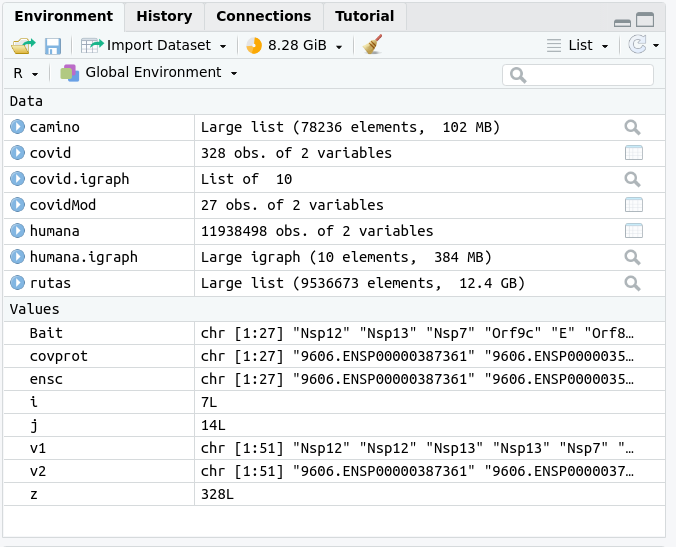
\includegraphics[scale = 0.3]{figures/allSimplePathTodos.png}
	\caption{Captura del tamaño de rutas creadas,sin compilacion completa con función all simple paths}
\end{figure}

\begin{figure}[ht!]
	\centering
	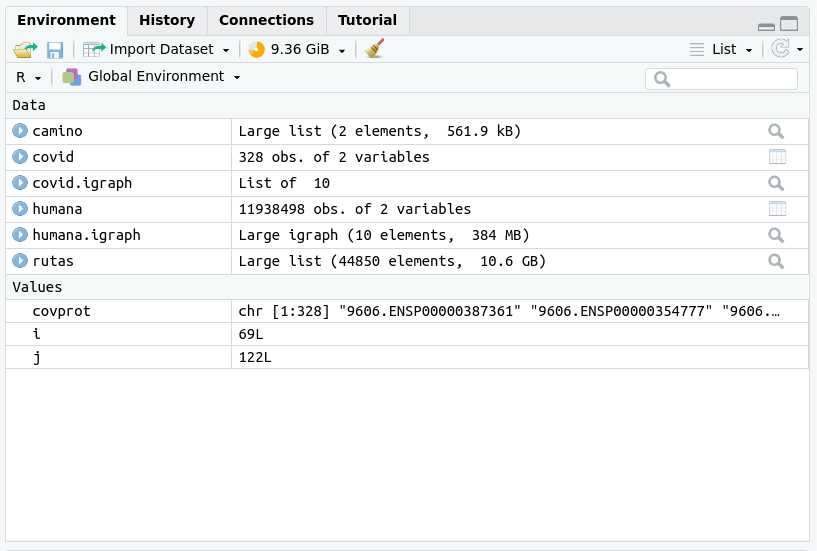
\includegraphics[scale = 0.3]{figures/allShortestPathTodos.png}
	\caption{Captura del tamaño de rutas creadas,sin compilacion completa con función all shortest paths}
\end{figure}



\subsection{Analisis de propiedades del grafo obtenido}
Realizaremos un analisis exahustivo de la red obtenida, analizando las propiedades estudiadas en clase.

\subsubsection{Comparacion entre la red obtenida y la red humana}
Encontramos los resultados de esta parte en la carpeta code y el codigo AnalisisRedFinal.R. Se estudian las siguientes componentes:
- Densidad: es considerada como una medida de cohesion entre los nodos de la red. Es una medida del numero de vinculos existentes en la red, presentados como una proporcion del numero de vinculos posibles. 
  * Densidad red proteoma humano: 0.03
  * Densidad red obtenida: 0.002
- Reprocidad: es una medida de probabilidad de que los vértices de una red dirigida se vinculen mutuamente entre sí. En general las redes reales tienen una reprocidad entre 0 y 1. Obtenemos un 1 para ambas redes.
- Diametro: se denomina asi al máximo camino más corto entre dos nodos medido por el numero de elnaces recorrido. Un diametro menor indica mayor habilidad de comunicacion en la red. Debe preocurarse que el diametro de las redes de intercomunicación sea lo más pequeño posible. 
  * Diametro red proteoma humano: 5
  * Diametro red obtenida: 7
  
  \begin{figure}[ht!]
	\centering
	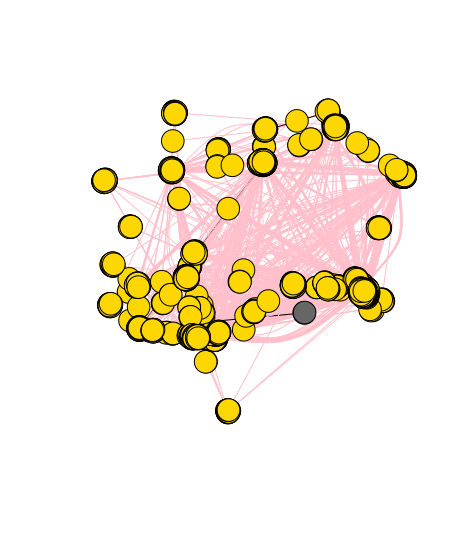
\includegraphics[scale = 0.3]{Rplot01.png}
	\caption{Representacion del diametro de la red conseguida}
\end{figure}

- Grado: es el número de conexiones de un vertice o nodo con otros nodos. 
  * Grado maximo red proteoma humano: 15014, solo para un nodo
  * Grado minimo red proteoma humano: 2, para 16 nodos
  * Grado maximo red obtenida: 620, solo para un nodo
  * Grado minimo red obtenida 1, parao 208 nodos
- Distribución de grado: la distribución de grado en una red representa habitualmente como P(K) y es definida como la fraccion de nodos en la red con un cierto grado k. 
- Distancia media: es el promedio o media de las distancias entre vertices en un grafo conexo, es una medida natural de la compacidad del grafo. 
  *Distancia media red proteoma humano: 2.040557
  *Distancia red obtenida: 3.517751
- Asortatividad: es la preferencia de los nodos de una red por unirse a otros que le son similares en alguna caracteristicas. Habitualmente se estudia en funcion del grado.
  *Asortatividad red proteoma humano: 0.1040102
  *Asortatividad red obtenida:-0.55738

\subsubsection{Modularidad}

Para obtener la modularidad del grafo hemos usado el paquete igraph. El codigo correspondiente se encuentra en un archivo llamado Modularidad y Centralidad.R
Lo primero fue obtener los modulos del grafo mediante la función cluster walktrap. Obtuvimos 68 grupos de tamaño diverso, desde 4 hasta 1778. Una vez obtenido esto, se le pasa a la funcion modularity transformándolo a un vector de membership (con la funcion membership) y pasando el grafo original como parámetro. El resultado es una modularidad de 0.935.
Despues de esto, representamos algunos valores pertinentes, como una lista de los tamaños de los grupos y Grafo en el que solo se ven los modulos coloreados.
Este grafo se hizo con plot.igraph, y nos muestra los 68 modulos por separado.
Aparte, vimos la posibilidad de representar un dendograma, pero no aporta ninguna informacion util debido a la cantidad de datos.


\subsubsection{Centralidad}

Tras realizar el an\'alisis de componentes, se ha observado que el m\'etodo de centralidad ganador ha sido el de \textbf{cercan\'ia}(closeness) de \textit{Spearman}. Dicho método considera como importancia aquellos nodos que están más cercanos de media al resto de nodos.
Una vez escogido el m\'etodo de closeness, se ha realizado el estudio de la centralidad con la funci\'on \textit{closeness} del paquete \textbf{igraph}. Dicha funci\'on nos ha otorgado la centralidad de cada nodo respecto al sistema de manera normalizada(Valores de entre cero y uno).
Analizando estos resultados, se ha obtenido que la media de la centralidad de los nodos de la red es \textbf{0.287}.
Adem\'as se ha calculado cuantos nodos de la red usada(subgrafo de la red que forma una sola componente conexa) tienen ciertos valores de centralidad.
En primer lugar, ho hay ningún valor de centralidad menor que 0.1. Con un valor de centralidad entre 0.1 y 0.3 hay un total de 1990 nodos, mientras que hay 898 nodos que presentan un valor de modularidad de entre 0.3 y 0.5. Por último, no hay ningún nodo con un valor de centralidad mayor de 0.5.


\subsubsection{Robustez}

Para comprobar la robustez de nuestro grafo vamos a realizar dos ataques dirigidos, uno basado en degree y otro en betweenness. En ambos casos representaremos el numero restante de nodos conexos por cada ataque en una grafica. Tras obtener los resultados, podemos observar que el ataque basado en betweenness deshace el grafo mucho mas rapido que el de degree. Esto tiene sentido ya que eliminar nodos clave con muchas uniones es muy eficaz. De hecho podemos ver que con el primer ataque ya reducimos la red de 9000 nodos a poco mas de 3000. Por tanto podemos deducir que hay un solo nodo que unia varios grupos de gran tamaño.
El ataque por degree es mucho mas gradual, pero aun asi deshace el grafo en aproximadamente 35 ataques.

\subsection{Enriquecimiento funcional}

El enriquecimiento funcional realizado est\'a en dos tablas distintas, una para cada columna de la tabla de genes que forma nuestro subgrafo.\newline
\begin{figure}[ht!]
	\centering
	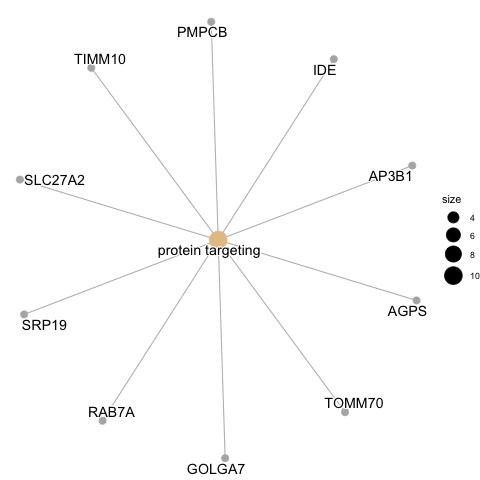
\includegraphics[scale = 0.2]{figures/GenesProteinTargeting.png}
	\caption{Genes que participan en \textit{Protein Targeting, GO:0006605}}
\end{figure}
De las dos tablas obtenidas observamos que la primera solo contiene una fila de un t\'ermino GO que es un proceso biol\'ogico. Dicho t\'ermino es \textbf{GO:0006605} y es un proceso biol\'ogico que hace referencia a orientar a prote\'inas espec\'ificas a regiones particulares de una c\'elula, normalmente a \'organulos celulares delimitados por membrana.
En la segunda tabla tenemos una gran multitud de t\'erminos de \textit{GO} apuntados. En total hay 2120 t\'erminos de los cuales 1586 son \textit{procesos bi\'ologicos}, otros 237 son \textit{funciones moleculares} y los \'ultimos 297 son \textit{componentes celulares}.\newline
En este caso como nos encontramos con una gran cantidad de t\'erminos no los nombraremos uno por uno sino que se mostrar\'an los t\'erminos que se consideren m\'as importantes mediante un diagrama de barras como con una red con las principales funciones. \newline
\begin{figure}[ht!]
	\centering
	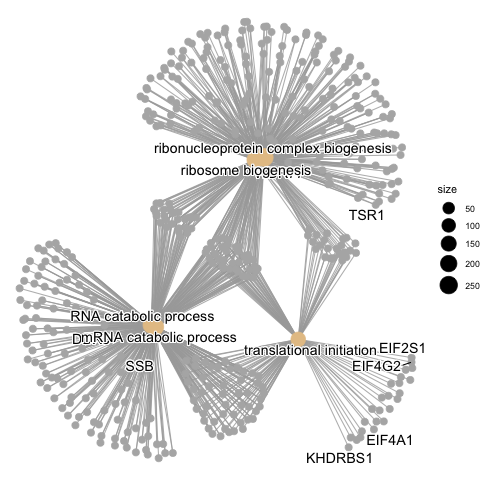
\includegraphics[scale = 0.2]{figures/Genes2Funciones.png}
	\caption{Red de funciones principales del segundo vector de genes}
\end{figure}

\begin{figure}[ht!]
	\centering
	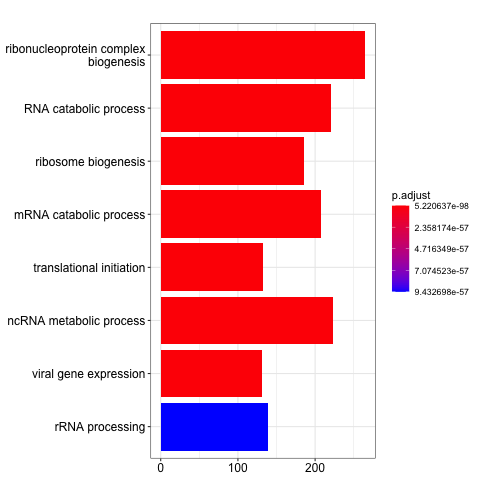
\includegraphics[scale = 0.3]{figures/barplotGenes2.png}
	\caption{Diagrama de las funciones m\'as importantes}
\end{figure}
\clearpage


	\section{Discusión}

\subsection{Datos a emplear}
Tras comparar los resultados de los tres algoritmos anteriores. Vemos que la tabla final que deberemos usar para el analisis se obtiene usando el tercer metodo, donde no perdemos ninguna proteina virica y unicamente perdemos 4 de las humanas. 
Ya que usando el metodo de biomaRt perdemos 225 genes humanos, perdemos tambien 4 genes viricos pertenecientes al Covid. Y hemos comprobado que usando bitR solo obteniamos 18 de las 332 proteinas humanas y además unicamente dos de las proteinas covid. 

\subsection{Grafo conexo}
Despues de todos los intentos por obtener un grafo conexo, mencionados en el apartado de resultados. Hemos conseguido obtener el grafo conexo, puede que no sea el grafo optimo ni contenga todas las rutas, debido a los diferentes problemas vistos, pero hemos conseguido unir mediante rutas de proteinas humanas, las proteinas del Covid. 
Hemos podido comprobar que el grafo del proteoma total formaba una unica componente conexa, por tanto todas las proteinas se encuentran en el mismo lugar, y pueden usarse las funciones de igraph para conseguir las rutas. 
Tambien se podria haber utilizado las matrices de adyacencia para obtener rutas, tal y como se vio en clase de teoria, pero preferimos haber optado por el metodo del uso de funciones del paquete igraph. La funcion empleada para ver si el grafo obtenido es conexo es components, donde su parametro no indica el numero de componentes, y su parametro csize indica el numero de vertices diferentes. 
Por tanto, obtenemos una red formada por 2888 nodos, 9333 enlaces entre ellos y una unica compoente conexa. De la cual podremos analizar su modularidad y analisis funcional.

\subsection{Comparacion entre la red obtenida y la red humana}
Vistos los resultados de la comparación podremos comentar lo siguiente:
- Vemos que la red de proteoma humana es más densa, por tanto, contiene muchas más conexiones entre nodos que la nueva creada.
- Observamos que la red del porteoma humana tiene caminos mas cortos entre si que la red obtenida, consiguiendo asi una red menos compacta.
- Aqui observamos una de las propiedades de las redes reales donde vemos que tenemos unos pocos nodos de alto grado y muchos nodos de grado mas bajo. 
- Una característica destacable es que en la red humana los nodos con el mismo grado tiende a undirse entres si, pero en nuestra red obtenida la asortatividad es muy baja.
- La distribución de grado es más o menos similar en ambas, y no siguen una distribucion binomial que corresponde a grafo aleatorios. Sino que la frecuencia va aumentando con el grado, para que asi se puedan ir formando los denominados hubs.
\subsection{Centralidad obtenida}
Tras realizar un breve an\'alisis de la centralidad de nuestro modelo usado(hay que recordar que estamos usando un subgrafo que forma una sola componente conexa, porque todo el grafo entero como componente conexa tiene un costo computacional demasiado elevado), hemos obtenido resultados que no eran del todo esperados.\newline
Recapitulando, los valores obtenidos se han normalizado mediante la funci\'on \textbf{closeness} que obtiene la centralidad, es decir, todos los valores de centralidad est\'an comprendidos entre 0 y 1. En primer lugar, hemos obtenido una media de centralidad de 0.287, n\'umero que puede ser considerado muy bajo, dado que podr\'ia llegar hasta 1. Esto quiere decir que probablemente gran parte de nuestros nodos del subgrafo carezcan de importancia dentro de este seg\'un su posici\'on relativa en el subgrafo. Tambi\'en se podr\'ia interpretar como que hay bastantes nodos distanciados del resto de nodos en la red, por lo que la componente conexa que tenemos podr\'ia estar muy dispersa.\newline
Por un lado, no tenemos ning\'un nodo con una centralidad menor de 0.1, sin embargo, la mayor\'ia de los nodos(1990) tienen una centralidad comprendida entre 0.1 y 0.3. Esto nos ayuda a reafirmar que la mayor\'ia de los nodos de la red poseen una centralidad baja. Teniendo en cuenta que estamos midiendo la centralidad con la cercan\'ia, y sabiendo que la centralidad de cercan\'ia de un nodo se calcula como $1/(\Sigma(d(i,j)), i != j)$, tenemos que cuanto mayor sean las distancias de un nodo al resto de nodos, menor centralidad tendr\'a. Dicho de otro modo, la mayor\'ia de los nodos poseen una distancia al resto de nodos bastante elevada.\newline
Por otro lado, aunque hay unos cuantos nodos(898) con un valor de centralidad de entre 0.3 y 0.5, no hay ninguno cuyo valor de centralidad sea mayor que 0.5, lo que nos quiere decir que no hay ning\'un nodo en nuestro subgrafo que pueda ser considerado central o importante. Esto puede deberse, o bien a que el subgrafo generado no consiga representar adecuadamente al grafo conexo original, o bien, simplemente los nodos tanto de nuestro subgrafo, como del grafo original est\'an demasiado dispersos entre ellos como para considerar que la centralidad y la importancia que tienen dentro de la red es suficientemente alta.


	\section{Conclusiones}
Para este trabajo de investigacion conseguimos obtener un grafo de las cualidades deseadas, quizas no contiene los caminos mas optimos, pero debido al gran tiempo y memoria de ejecucion se ha simplificado hasta poder obtener uno lo suficientemente sencillo y completo. Este nos permite obtener, mediante cluster profiler, las funciones en las que intervienen nuestras proteinas y las componentes de las que forman parte. Tras el analisis realizado, vemos que obtenemos caracteristicas de las redes reales y no de redes aleatorias. \newline

A partir de este grafo hemos podido obtener mucha información que podria ser relevante a la hora de expandir en esta investigación, como podría ser la alta modularidad observada.
Esto podriamos haberlo supuesto por el contexto del proyecto, pero un resultado inesperado fue lo efectivo que seria un ataque dirigido mediante betweenness. El breakdown point se encuentra al incio del ataque, tan solo en el tercer ataque la red se deshace en un 90 porciento. Esto podria deberse a la presencia de una o varias proteinas esenciales para gran parte de los procesos de la red, y por tanto al eliminarla bloqueamos dichos procesos.\newline

Adem\'as, la centralidad de dicho subgrafo es bastante baja de media, y teniendo en cuenta que ha sido calculada por cercan\'ia, podemos afirmar que la mayor\'ia de nodos se encuentran distanciados entre ellos. 
Por \'ultimo, hemos obtenido que las funciones principales en las que se involucran los genes de nuestro subgrafo son principalmente la s\'intesis de complejos de ribonucleoprote\'inas y de ribosomas, procesos que pueden ser considerados esenciales en la s\'intesis de copias del virus. De esta manera podemos decir que los genes que tenemos tienen un gran importancia en el desarrollo del Coronavirus dentro de la c\'elula.


	
	
	%%%%%%%%%%%%%%%%%%%%%%%%%%%%%%%%%%%%%%%%%%%%%%
	%% OTRA INFORMACIÓN                         %%
	%%%%%%%%%%%%%%%%%%%%%%%%%%%%%%%%%%%%%%%%%%%%%%
	
	\begin{backmatter}
	
		\section*{Abreviaciones}%% if any
			Indicar lista de abreviaciones mostrando cada acrónimo a que corresponde
		
		\section*{Disponibilidad de datos y materiales}%% if any
			https://github.com/Joseantoniomr99/project_template.git
		
		\section*{Contribución de los autores}
			E.M.S : Encargada de generar con bitR el grafo del proteoma del score 800-950, analisis de mejor forma de uso para cambiar del tipo de 
			datos de proteinas iniciales a tipo de datos string para conicidir con proteoma, obtención de datos para creacion de red,
			creacion del grafo conexo de union de proteinas covid con proteinas humanas, memoria de latex de los codigos anteriores mencionados.
		
		
		%%%%%%%%%%%%%%%%%%%%%%%%%%%%%%%%%%%%%%%%%%%%%%%%%%%%%%%%%%%%%%%%%%%%%%%%%%%%%%%%%%%%%%%%
		%% BIBLIOGRAFIA: no teneis que tocar nada, solo sustituir el archivo bibliography.bib %%
		%% por el que hayais generado vosotros                                                %%
		%%%%%%%%%%%%%%%%%%%%%%%%%%%%%%%%%%%%%%%%%%%%%%%%%%%%%%%%%%%%%%%%%%%%%%%%%%%%%%%%%%%%%%%%
		
		\bibliographystyle{bmc-mathphys} % Style BST file (bmc-mathphys, vancouver, spbasic).
		\bibliography{bibliography}      % Bibliography file (usually '*.bib' )
	
	\end{backmatter}
\end{document}
